\documentclass{beamer}


\graphicspath{{figures/}}
\usepackage{tikz}
%\usetheme{boxes}
\usepackage[utf8]{inputenc}
\usepackage{amsmath}
\usepackage{amsthm}
\usepackage{hyperref}
\usepackage[font=tiny]{caption}
\usepackage{booktabs}
\usepackage{natbib}
\bibliographystyle{plainnat}
\usecolortheme{crane}

\definecolor{orange}{RGB}{232, 86, 15}
\definecolor{blue}{RGB}{14, 159, 232}
\definecolor{blueblue}{RGB}{50, 90, 160}
\definecolor{yellow}{RGB}{232, 187, 14} 
\definecolor{red}{RGB}{232, 14, 59}

\hypersetup{
  colorlinks=true,
  linkcolor=cyan,
  urlcolor=cyan,
  citecolor=purple
}
\newtheorem{deff}{Definición}
%Information to be included in the title page:
\institute[]{}

\setbeamercolor{title}{bg=blueblue, fg=white}
\setbeamercolor{subttile}{bg=blueblue, fg=white}
\setbeamercolor{frametitle}{bg=blueblue, fg=white}
\setbeamercolor{block title}{bg=blue, fg=white}
\setbeamercolor{block title alerted}{bg=red, fg=white}
\setbeamercolor{block title example}{bg=yellow, fg=white}
\setbeamercolor{footline}{bg=gray, fg=white}

\beamertemplatenavigationsymbolsempty

\title{Gherardo Varando}
\author{Gherardo Varando}
\date{25 March 2025}
\begin{document}

\begin{frame}{(Casual) Causality Course 2025}

	\begin{block}{Intructors}
	  \begin{itemize}
	    \item Gherardo \url{gherardo.varando@uv.es}
	    \item Emiliano \url{emiliano.diaz@uv.es} 
	    \item Vassilis \url{vasileios.sitokonstantinou@uv.es}
	  \end{itemize}
	\end{block}
	
	\begin{block}{Schedule} 
         \begin{itemize}
	   \item \textbf{week 1, Tuesday} Intro and causal inference (GV)
	   \item \textbf{week 1, Thursday} Causal inference and robustness (GV)    
	   \item \textbf{week 2, Tuesday} Causal Discovery (ED)
	   \item \textbf{week 2, Thursday} Causal Discovery (ED)
	   \item \textbf{week 3} Intensive weeek with group projects! 
	 \end{itemize}
	\end{block}


\end{frame}


\begin{frame}{Learning outcomes} 

  \begin{columns}
    \begin{column}{0.5\textwidth}
  \begin{itemize}[<+-|alert@+>]
    \item Understand the fundamental
          goals and problems of causal methods  
    \item Familiarize with the vocabulary, definitions and basic concepts of causality
    \item Understand the fundamentals behind basic methodologies in
          causal inference and causal discovery
	\item How causal methods and tools are relevant in ML?
  \end{itemize}
    \end{column}
    \begin{column}{0.5\textwidth}
      \only<1>{
	\begin{figure}
	  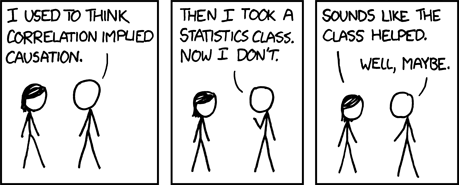
\includegraphics[width=5cm]{correlation}
	  \caption{xkcd (CC BY-NC 2.5) \url{https://xkcd.com/552}}
	\end{figure}
      }
\only<2>{
	\begin{figure}
	  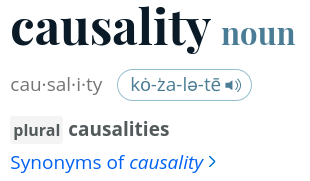
\includegraphics[width=5cm]{causality_noun}
	  \caption{\url{https://www.merriam-webster.com/dictionary/causality}}
	\end{figure}
      }
\only<3>{
	\begin{figure}
	  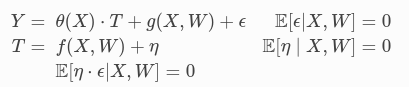
\includegraphics[width=5cm]{dml}
	  \caption{\url{https://econml.azurewebsites.net}}
	\end{figure}
      }
 \only<4>{
	\begin{figure}
	  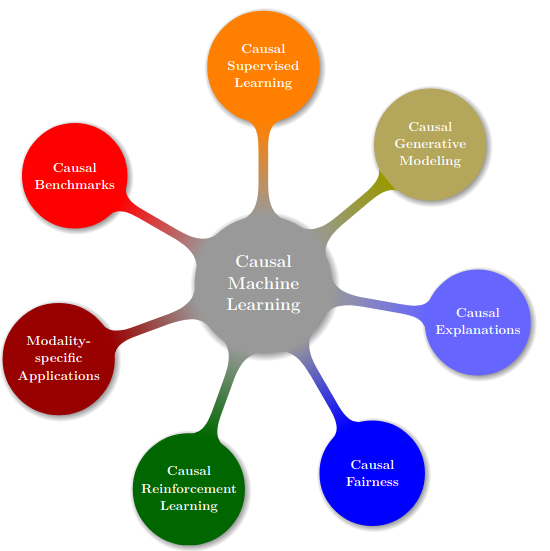
\includegraphics[width=5cm]{causal_ml}
	  \caption{From \cite{kaddour2022causalmachinelearningsurvey}}
	\end{figure}
      }
    \end{column}
  \end{columns}
\end{frame}

\begin{frame}{Content week 1}
  \begin{itemize}
    \item \textbf{Session 1} Tue 25/03
      \begin{itemize}
	\item[Part I] \textbf{Intro to causality and causal methods} \\ 
	  \only<2>{motivation, causal questions, what is causality? \\
		      experiments, interventions and counterfactuals \\ 
		      structural causal models and graphs}
         \item[Part II] \textbf{Basics of causal inference} \\
	     \only<2>{causal effect, randomized experiments  \\
	              observational studies, identifiability conditions \\
		      graphical representation, confounding, selection bias \\
		      random variability and measurement error 
	   } 
      \end{itemize}
\vfill
    \item \textbf{Session 2} Thu 27/03
      \begin{itemize}
	\item[Part I] Causal inference methods
	\item[Part II] Robustness to interventions  
      \end{itemize}
  \end{itemize}
\end{frame}

\begin{frame}{Basic references}
  \begin{itemize}
    \item \href{https://mitpress.mit.edu/9780262037310/elements-of-causal-inference/}{Elements of causal inference} \citep{peters2017elements} [EC] 
    \item \href{https://miguelhernan.org/whatifbook}{Causal Inference: What If} \citep{hernan2025causal} [Wif]
    \item All of Statistics \citep{wasserman2013all} [AoS] 
  \end{itemize}

  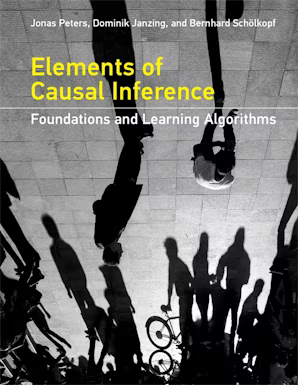
\includegraphics[width = 2 cm]{elements}
  
\includegraphics[width = 2 cm]{whatif}
  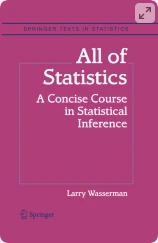
\includegraphics[width = 2 cm]{all}
\end{frame}


\begin{frame}{}


  \begin{columns}
    \begin{column}{0.8\textwidth}
  \begin{quote}
Felix qui potuit rerum cognoscere
causas \dots \\
    \hfill \small \textnormal{Publius Vergilius Maro \\ \hfill Georgica \href{https://www.poetryintranslation.com/PITBR/Latin/VirgilGeorgicsII.php}{Book Two}}
  \end{quote}
      \onslide<2>{
	\centering
	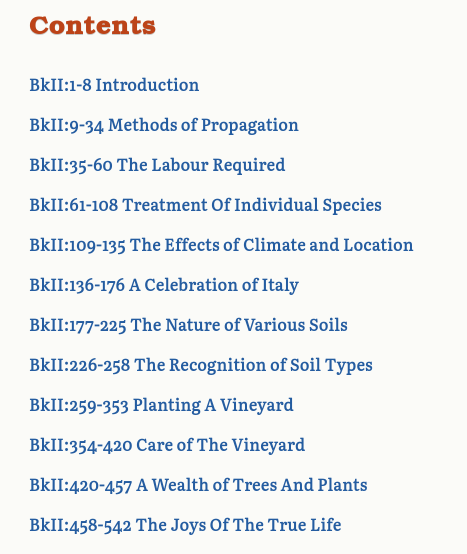
\includegraphics[scale=0.3]{book2index}
      }
    \end{column}
    \begin{column}{0.4\textwidth}
      \begin{figure}
	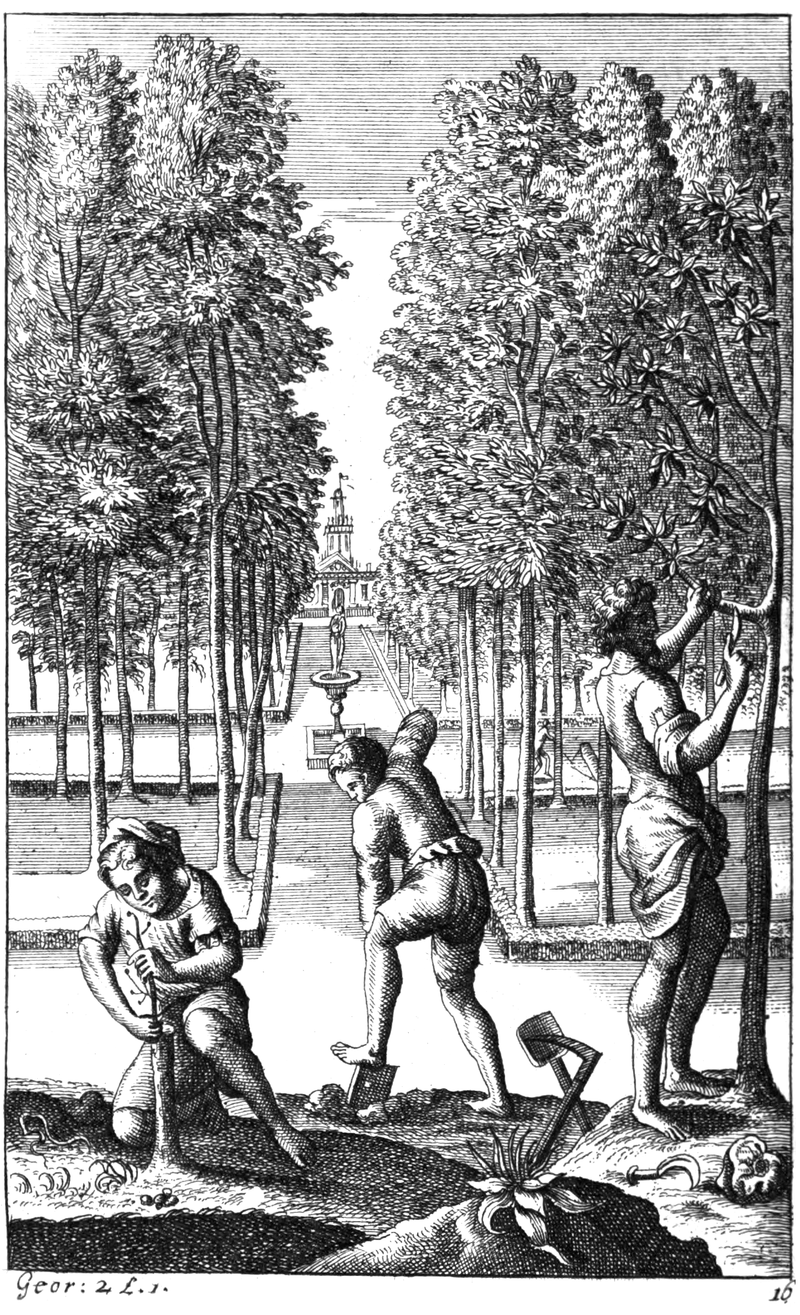
\includegraphics[scale=0.18]{book2}
	\caption{By Michael van der Gucht - \href{https://commons.wikimedia.org/w/index.php?curid=88226096}{Public Domain}}
      \end{figure}
    \end{column}
  \end{columns}
\end{frame}

\begin{frame}{What is causality?}
  \begin{columns}
    \begin{column}{0.7\textwidth}
  %\begin{center}
  %  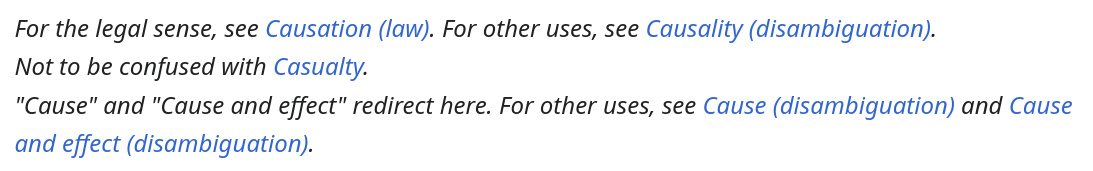
\includegraphics[width=0.95\textwidth]{Causality-Wikipedia}
  %\end{center}
  \begin{itemize}
    \item Causality in Law  \url{https://en.wikipedia.org/wiki/Causation_(law)} \\
      \href{https://www.youtube.com/watch?v=XiCOmhdkM80&list=PLqMxKp2ot-3vDaLyaAZNgt8ijj6n0l460}{Causation|Low of Tort playlist on youtube, first 3 videos}  
    \item Causality in Physics \\
       \url{https://en.wikipedia.org/wiki/Causality_(physics)}  \\
       \url{https://www.youtube.com/watch?v=eG_eHDDMgCs} \\
       \cite{rovelli2022causationrootedthermodynamics}  
  \end{itemize}
  \end{column}
    \begin{column}{0.3\textwidth}
       \begin{figure}
	 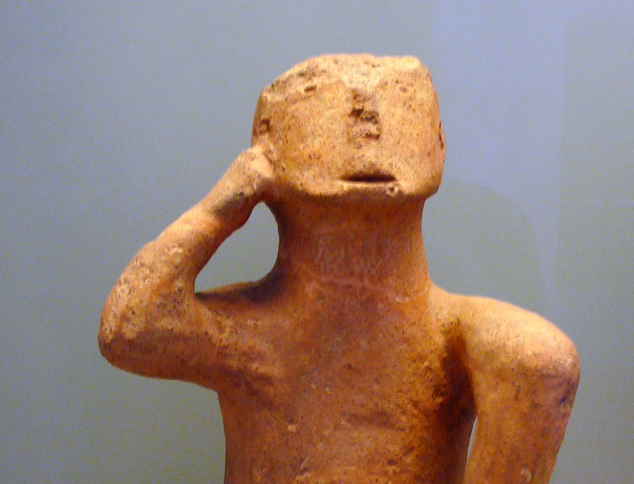
\includegraphics[width=3cm]{thinker1}
	 \caption{Karditsa Thinker at the National Archaeological Museum, Athens} 
       \end{figure}
       \vfill
    \onslide<2->{
      \begin{itemize}
	  \tiny
	\item Work in groups and briefly discuss causality in physics or law 
	      \textbf{[20 min]}
	\item  
      \end{itemize}
    }
    \end{column}
  \end{columns}
\end{frame}


\begin{frame}{Non-causal questions ... still important!!}
  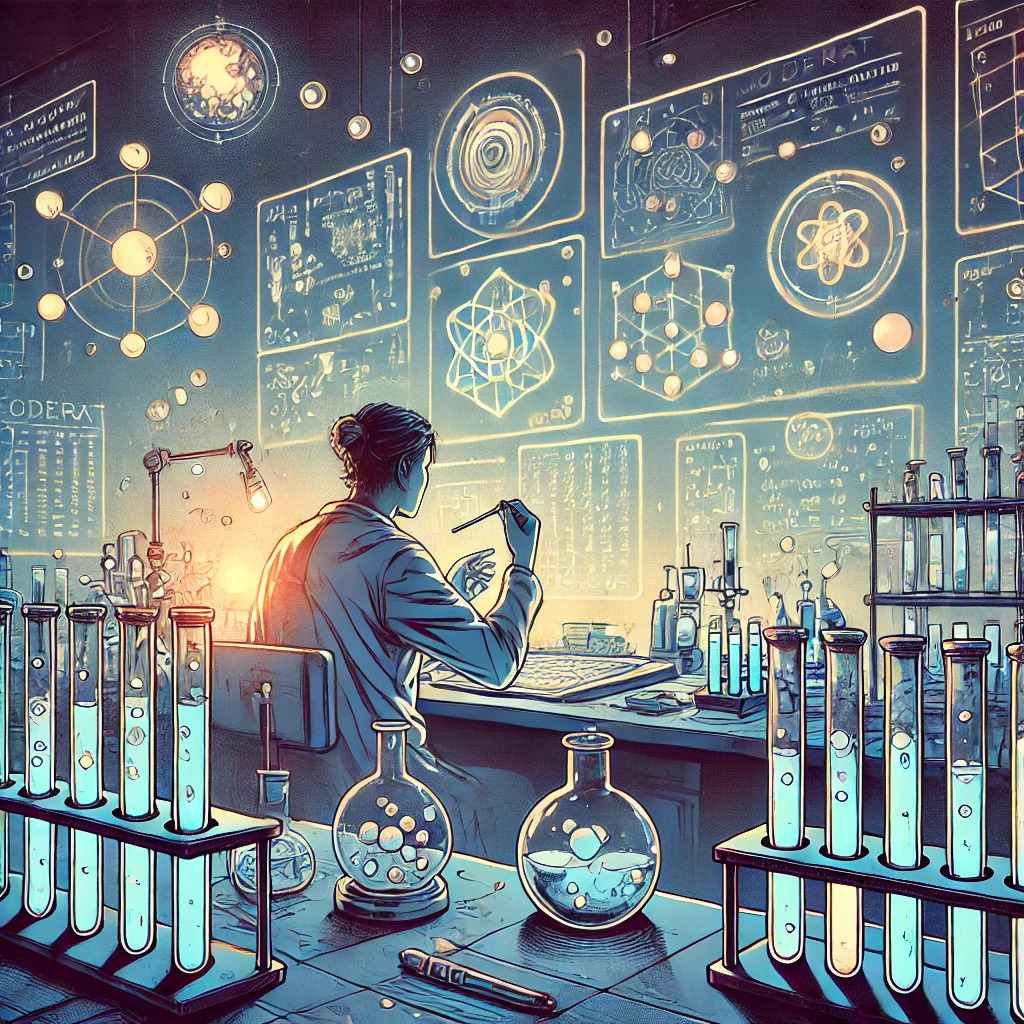
\includegraphics[width=0.45\textwidth]{scientist}
  
\includegraphics[width=0.45\textwidth]{QR0}
\end{frame}

\begin{frame}{Non-causal questions ... still important!!}
  \begin{columns}
    \begin{column}{0.5\textwidth}
      \begin{itemize}[<+-|alert@+>]
	\item Estimate the tree diameters or age in a forest \citep{west2021tamm} 
	\item Counts the number of trees in the desert
	  \citep[\href{https://www.nature.com/articles/s41586-020-2824-5}{unexpectedly high}][]{brandt2020unexpectedly} 
	\item Cloud detection \citep{aybar2024onboard} 
	\item Describing patterns of wood density \citep{yang2024} 
      \end{itemize}
    \end{column}
    \begin{column}{0.5\textwidth}
      \only<1>{
	\begin{figure}
	  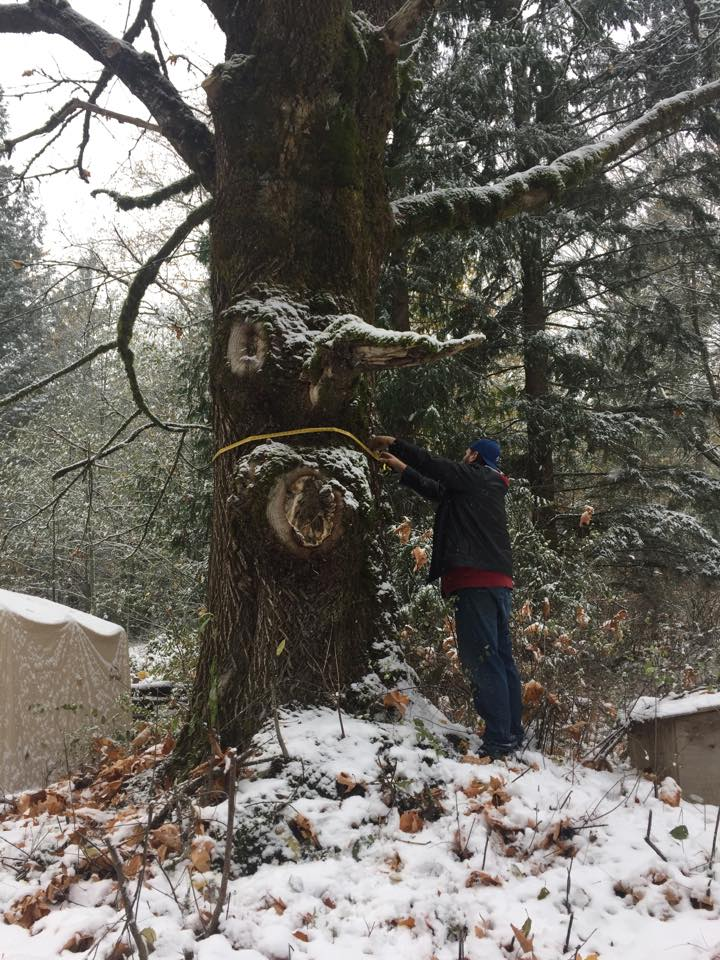
\includegraphics[width=4cm]{tree-meas}
	  \caption{From \url{https://theforestguild.com/estimating-the-age-of-trees/}}
	\end{figure}
      }
      \only<2>{
	\begin{figure}
	  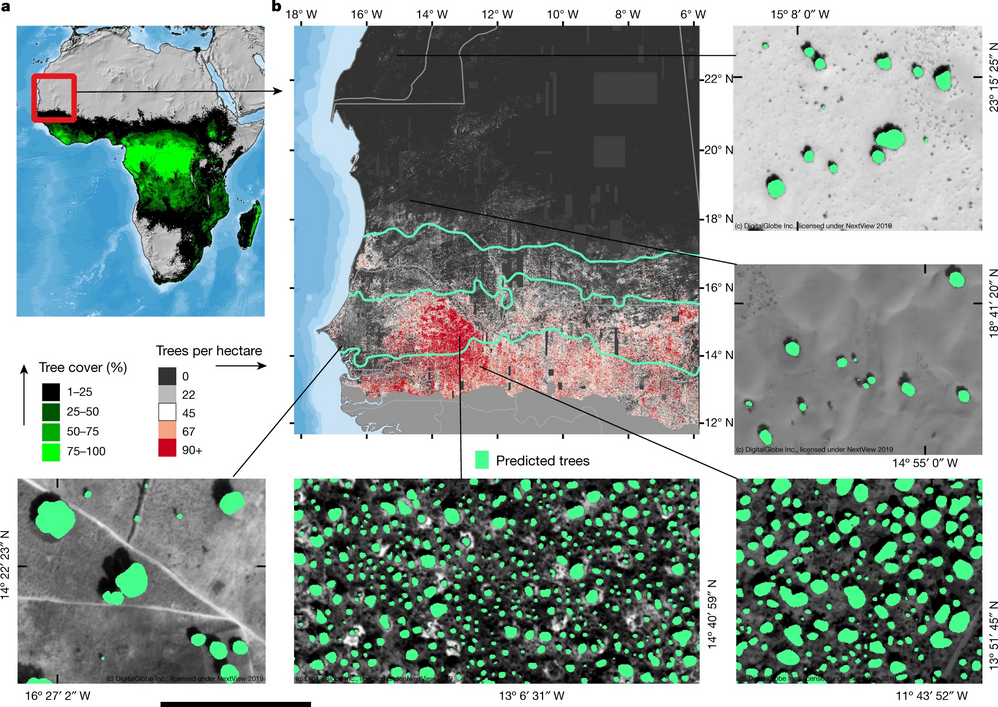
\includegraphics[width=6cm]{tree-desert}
	  \caption{From \cite{brandt2020unexpectedly} \href{https://www.nature.com/articles/s41586-020-2824-5}{paper}}
	\end{figure}
      }
      \only<3>{
	\begin{figure}
	  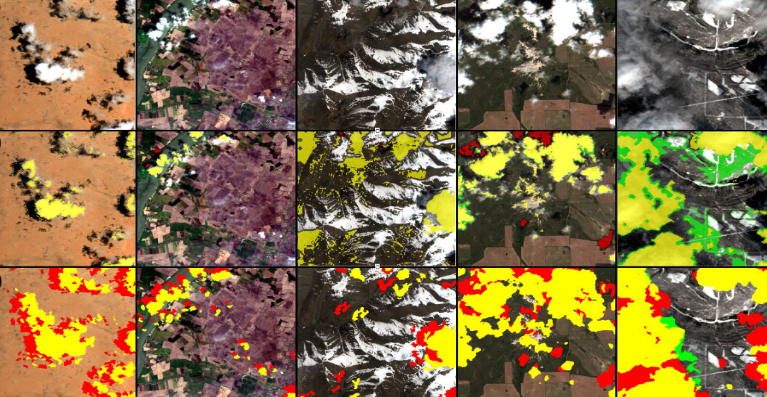
\includegraphics[width=6cm]{cloud}
	  \caption{From \cite{aybar2024onboard} \href{https://events.ecmwf.int/event/304/contributions/3629/attachments/2126/3769/ECMWF-ESA-WS_Garicia-Acciarini.pdf}{poster}} 
	\end{figure}
      }
      \only<4>{
	\begin{figure}
	  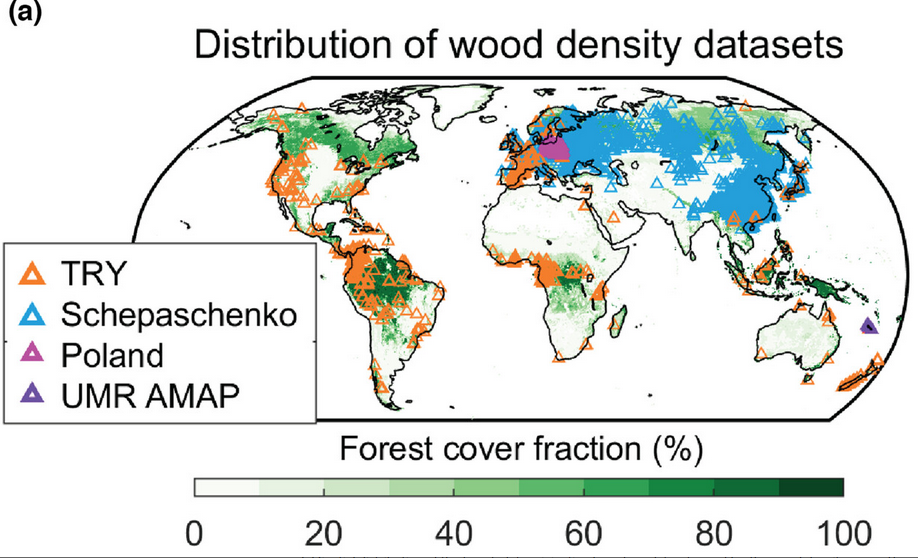
\includegraphics[width=6cm]{wood_density}
	  \caption{From \cite{yang2024} \href{https://onlinelibrary.wiley.com/doi/10.1111/gcb.17224}{paper}} 
	\end{figure}
      }
    \end{column}
  \end{columns}

\end{frame}


\begin{frame}{Causal questions}
  
\includegraphics[width=0.45\textwidth]{QR0}
  
\includegraphics[width=0.45\textwidth]{scientistthink}
\end{frame}

\begin{frame}{Causal questions}
  \begin{columns}
    \begin{column}{0.5\textwidth}
      \begin{itemize}[<+-|alert@+>]
	\item How droughts affect yields 
	\item Evaluate agricultural practice \citep{tsoumas2023evaluating, Giannarakis_2022_CVPR} 
	\item How does armed conflict influence tropical forest loss? \citep{Christiansen03042022} 
	\item Estimate the effect of ENSO on vegetation \citep{le2023increased} 
      \end{itemize}
    \end{column}
    \begin{column}{0.5\textwidth}
      \only<1>{
	\begin{figure}
	  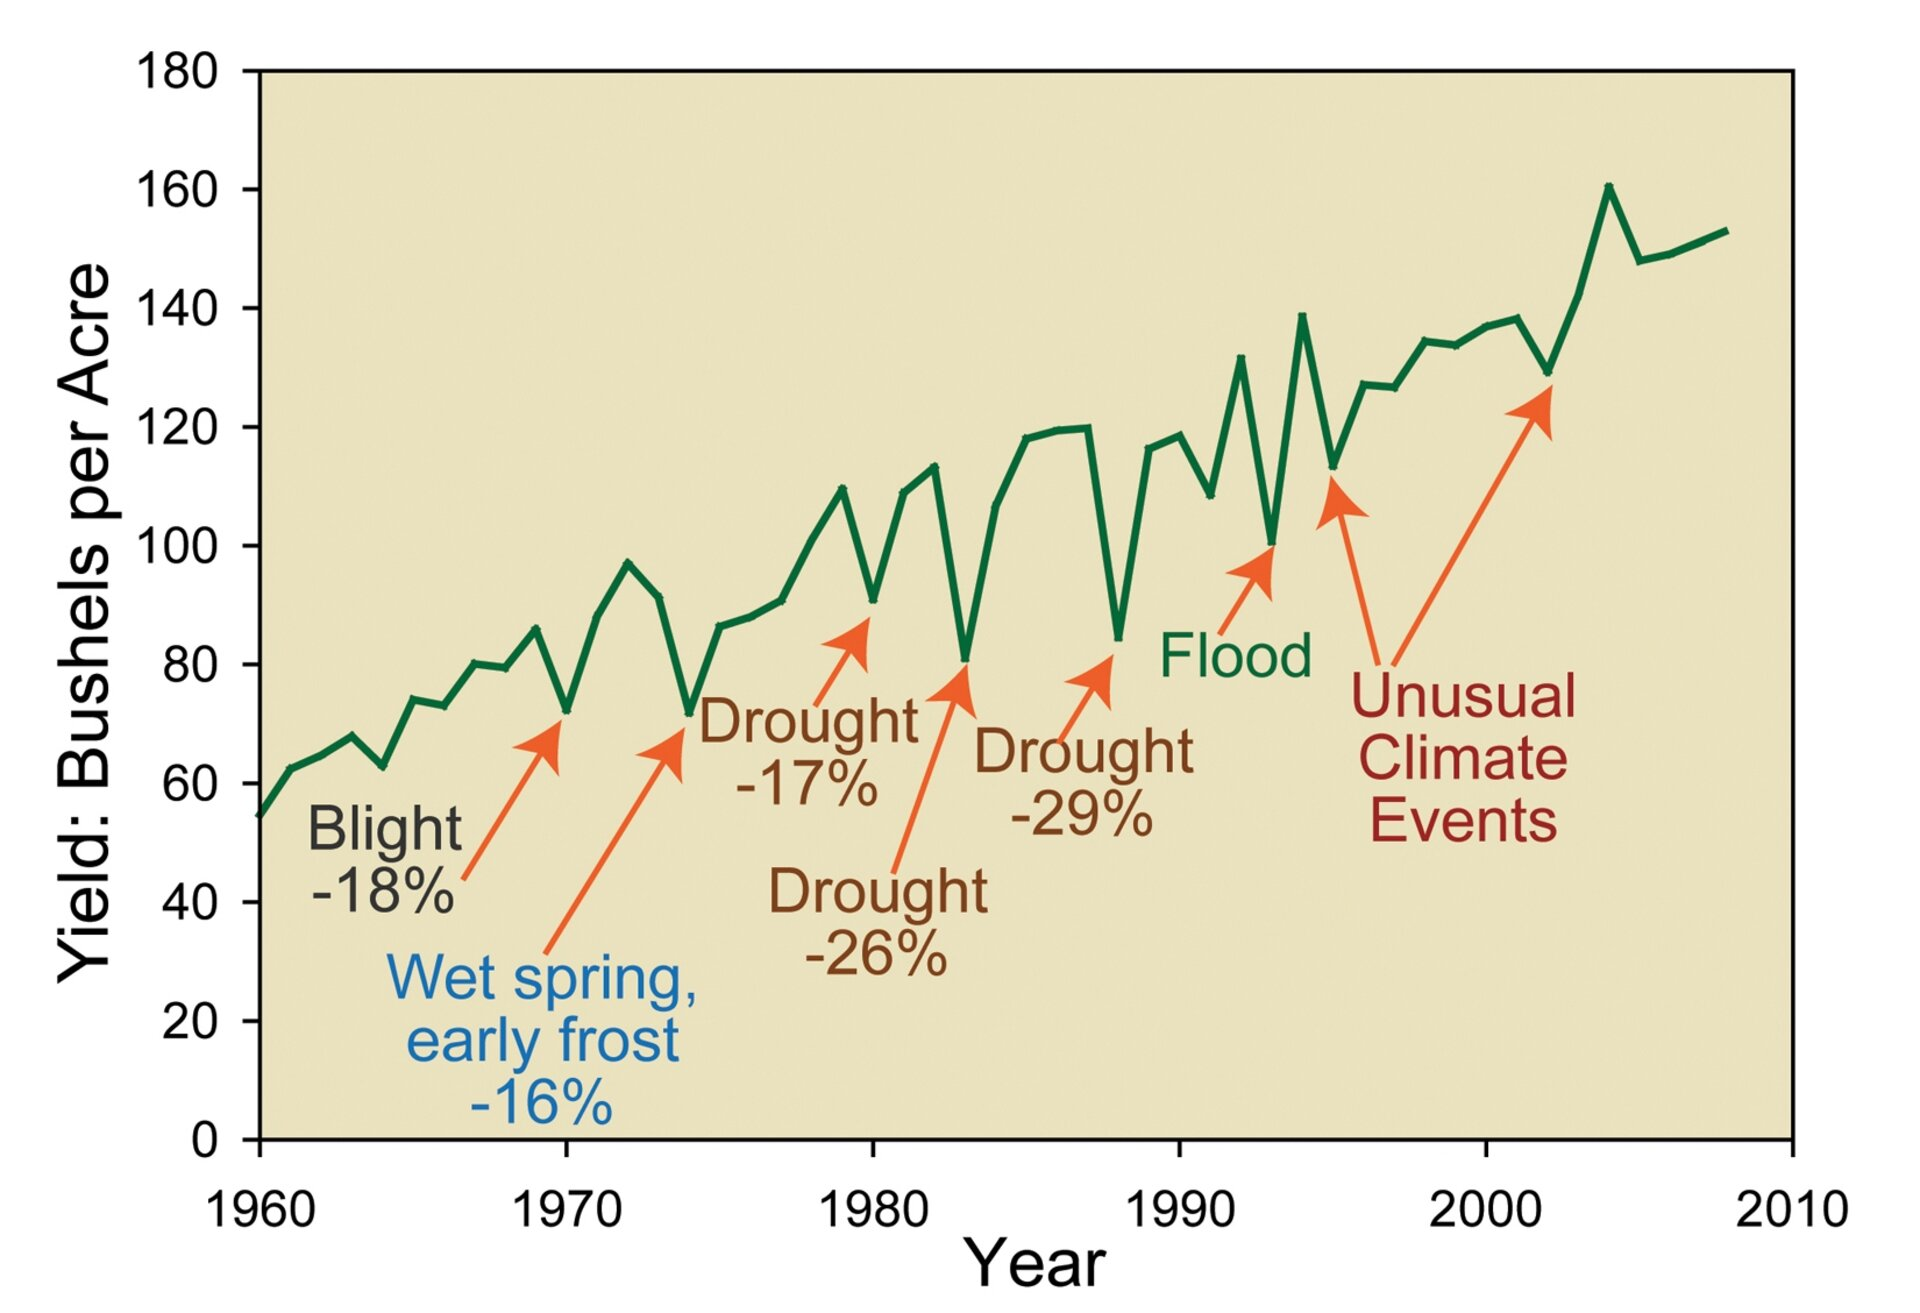
\includegraphics[width=6cm]{effect_drought}
	  \caption{credit USDA FAS, from \href{https://www.esa.int/ESA_Multimedia/Images/2014/05/Effect_of_drought_on_corn_yields}{ESA Website} (ESA Standard
Licence)}
	\end{figure}
      }
      \only<2>{
	\begin{figure}
	  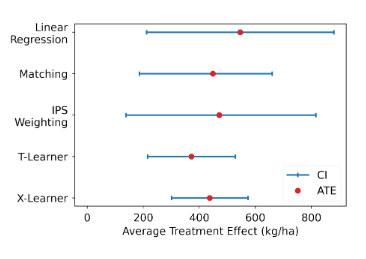
\includegraphics[width=6cm]{agri_effect}
	  \caption{From \cite{tsoumas2023evaluating}}
	\end{figure}
      }
      \only<3>{
	\begin{figure}
	  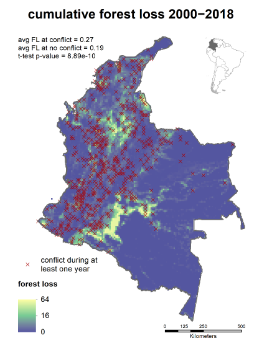
\includegraphics[width=4cm]{forest_loss}
	  \caption{From \cite{Christiansen03042022}} 
	\end{figure}
      }
      \only<4>{
	\begin{figure}
	  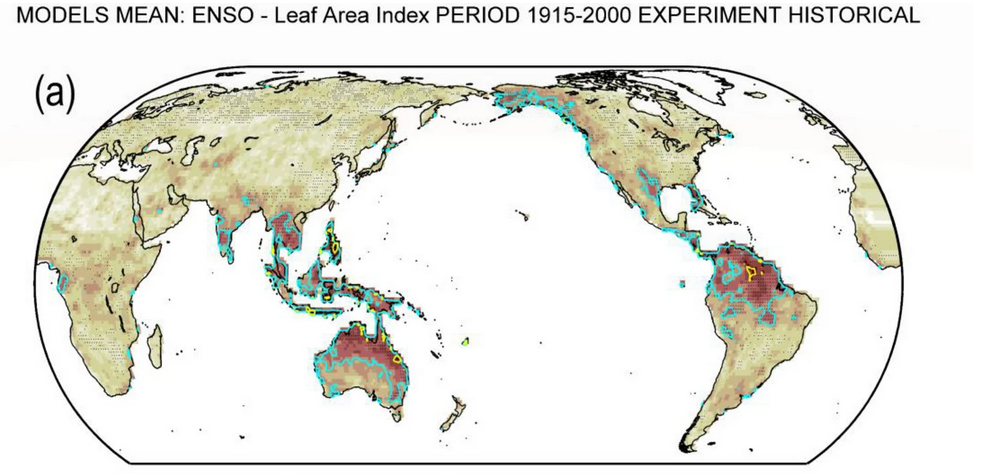
\includegraphics[width=7cm]{enso_veg}
	  \caption{From \cite{le2023increased}} 
	\end{figure}
      }
    \end{column}
  \end{columns}

\end{frame}


\begin{frame}{Probabilistic causation}

  \begin{block}{\citep[][AoS, Chapter 16]{wasserman2013all}}
    \begin{quote}
	Roughly speaking, the statement `` $X$ causes $Y$'' means that 
	changing the value of $X$ will change the distribution of $Y$.
      \end{quote}
  \end{block}
  \begin{itemize}
    \item<2-> How to make the previous \emph{definition} precise and operative? 
    \item<3-> What does it mean \text{changing the value} of $X$? 
    \item<4-> various solutions are possible, we will see two possibilities:
      \textbf{Structural Causal Models (SCM)} and the \textbf{Potential Outcome framework}
  \end{itemize}
\end{frame}


\begin{frame}{Structural Causal Models}


\end{frame}


\begin{frame}

\end{frame}



\begin{frame}{On the concept of \emph{Harm}} 
  \begin{itemize}
    \item \cite{sarvet2023perspective}  interventionalist vs contrefactual  
    \item \cite{mueller2024perspective} response 
  \end{itemize}
\end{frame}


\begin{frame}{Personalized decision making}
  \begin{itemize}
    \item \cite{mueller2023personalized} 
    \item \cite{tian2000probabilities} 
  \end{itemize}
\end{frame}


\begin{frame}[allowframebreaks]{Bibliography}
  \tiny
\bibliography{biblio}
\end{frame}

\end{document}


